\section{Feature tracking}
\label{sec:sec2_feature_tracking}

ESTA PARTE PRECISA DE TRABALHO, ESTOU UM POUCO INCERTO SE VALE A PENA INCLUIR SIFT E SURF (PELO MENOS DA FORMA COMO ESTÁ)

Having identified features, an important step is being able to match them or track them across multiple frames. As such, it is important to choose features which are unique and not easily mismatched (distinct features), as well as features that are easy to reidentify from multiple angles (robust and stable features, invariant to viewing direction and distance, and illumination variances).

A simple approach is to use a global minimization approach through the Sum of Squared Distances (SSD) between the features being proposed as a match, with the underlying principle that matching features are close to each other in consecutive frames. However, this is not always the case. Also, this approach complicates feature reidentification whenever it exits and re-enters the frame, and is also slow. This technique is better suited for template tracking across frames, assuming rigid body motion, which is not always the case, with independent feature movement.

To facilitate feature matching in classical cameras, along with the features detected (interest points), image descriptors around these points are also preserved, which are then compared for matching. This approach is used by Scale-Invariant Feature Transform (SIFT \cite{lowe1999object}), Speeded Up Robust Features (SURF \cite{bay2006surf}) and similar approaches.

\subsection{SIFT features}
\subsubsection{SIFT detection}
VALE A PENA FALAR DA DETECAO OU SO DOS DESCRITORES????

Features of interest are designated as keypoints in the SIFT framework. This detector uses blobs as keypoints, and relies on the Difference of Gaussians (DoG) to extract keypoints, which are invariant to translation, scaling and rotation.

A pyramid of images of different scales is generated, and for each scale, multiple convolutions with Gaussian kernels are performed (which effectively blurs the images). For each scale, a difference between images (Difference of Gaussians) is performed, and maximum and minimum across scales are kept.

\subsubsection{SIFT descriptors}

Each keypoint has a corresponding descriptor. For each keypoint, a grid of  4x4 blocks is created, each containing 4x4 sub-blocks. For each sub-block, its main orientation is estimated, and all 16 sub-block orientation are condensed into a bin with 8 directions. As such, each feature has a 4x4 blocks x 8 orientation bin which creates a 128D descriptor.

The relevance of the descriptors is when matching, since a variation of the k-d tree algorithm (called the best-bin-first search method) is used to compare and match keypoints fast and correctly across multiple frames.

\subsection{SURF features}
\subsubsection{SURF detection}
VALE A PENA FALAR DA DETECAO OU SO DOS DESCRITORES????

Features of interest detected using the determinant of the Hessian matrix (technique similar to the Harris corner detector), using the same pyramid approach.


\subsubsection{SURF descriptors}

Each keypoint has a corresponding descriptor. For each keypoint, a grid of  4x4 blocks is created, which record orientation using Haar wavelet functions. Each block registers 4 components, resulting in 4x4 grid x 4 components, resulting in a 64D descriptor for each keypoint.

These descriptors are then used for matching features across frames, like with SIFT.

\subsection{Event cameras}

ESTA PARTE JA ME PARECE MAIS ROBUSTA

For event cameras, a typical choice of features, as previously presented, are corners. However, the choice of descriptors for matching and tracking is not yet as developed as for classic cameras.

\subsubsection{SSD}

A first approach to feature matching across frames is to rely on the fast nature of events, and to create pseudo-frames by combining features over a timeslice (accumulation of events for a given interval). The features of both pseudo-frames can then be matched using SSD, assuming a proximity between features in consecutive pseudo-frames. 

Nevertheless, this approach is not ideal, as a critical parameter is the time of integration in the timeslice, which does not take full advantage of the nature of events and event cameras, and could be so slow as to have the same temporal resolution as conventional cameras.

\subsubsection{Spatiotemporal tracking}

The technique presented in Section\,\ref{sec:sec2_space_time} for corner detection is also able to track these corners across multiple timestamps, since the plane and line fitting that are performed in the spatio-temporal representation of events for edges and corners, respectively, implicitly estimates their motion and position across time.

However, since no descriptors or identifiers are being registered, some problems arise when features leave the camera space and are recaptured later, as well as situations where multiple corners overlap and end up merging together. This is particular true for corners from organic features, as opposed to artificial structures.


\subsubsection{EKLT}

EKLT (\cite{gehrig2020eklt}) is a hybrid feature tracking technique that is able to merge information from conventional cameras and events (and hence is more suitable for the new generation of DAVIS event cameras), that tracks corners across time. The method is based on the Lucas-Kanade tracker, hence the name EKLT (event-based Lunas-Kanade tracking).

This method tracks corners, as they are easy to recognize in both conventional cameras (Section\,\ref{sec:sec2_classic_corner_detection}), and correspond to areas with high event generation, that can be detected using event corner detectors as well (Section\,\ref{sec:sec2_sae_corner_detection}).

The idea behind this tracker is to detect features using a conventional frame, which are then tracked using events until a new frame arrives, at which point the estimation from events is compared to the corner detection in the new frame, in essence correcting this estimation. If the feature is not detected, it is still tracked in event space, as subsequent frames may re-detect missed features. This approach is particularly useful in high-speed movements, where motion blur becomes a problem for frames, but not for events.

This comparison between frames and events is crucial, and the key concept is "image variation in a frame patch". As previously discussed (Section\,\ref{sec:sec2_event}), event cameras respond to brightness changes in the environment. Therefore, it is not farfetched to compare events to image gradients, as zones with higher gradients in the world are precisely the ones that produce the most events. In fact, integration (accumulation) of events over a period of time produce results that are very similar to the gradient of the image, as shown in Fig.\,\ref{fig:sec2_gradient_comparison}.

\begin{figure}[ht]
	\centering
		\begin{tabular}{cc}
		   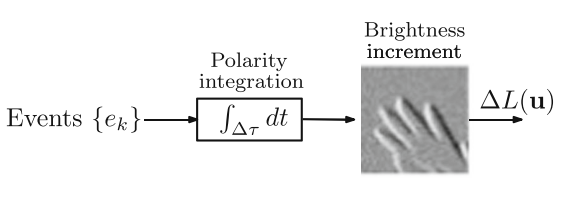
\includegraphics[width=0.45\linewidth]{gradient1.png} &
		   \hspace{1cm} 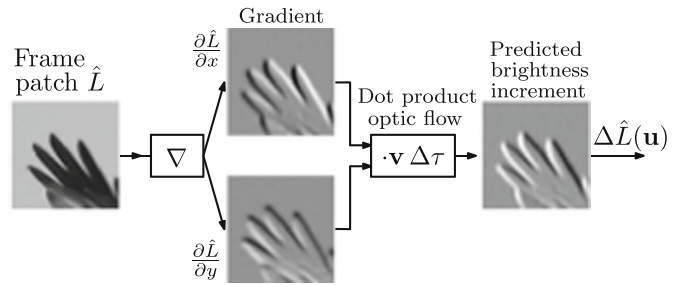
\includegraphics[width=0.45\linewidth]{gradient2.png} \\
		   (a) & (b)  \\
		\end{tabular}
	\caption[Comparison of the brightness change from event integration with the brightness change from image gradient]{Comparison of the brightness change from event integration (a), versus the brightness change from image gradient (b), from \cite{gehrig2020eklt}}
	\label{fig:sec2_gradient_comparison}
\end{figure}

This is the idea at the core of this approach, as the brightness change behaves as the descriptor for the features, and are used as patches for a Lucas-Kanade inspired patch comparison and matching, using both the patch and estimated velocity (estimated through events), using the cost function \eqref{eq:sec2_cost_eklt}, where $\Delta L$ denotes changes from events, $\Delta \hat{L}$ denotes gradients from frames, and $u$ denotes the image, $p$ the warp parameters, and $v$ the velocity. $p$ and $v$ are used as the starting values for the optimizer that minimizes the functional \eqref{eq:sec2_cost_eklt}, and are modified during the optimization process.

\begin{equation}
    \label{eq:sec2_cost_eklt}
    \min_{p,v} \left \| \Delta L(u) - \Delta \hat{L}(u,p,v)) \right \| ^2
\end{equation}

While a new frame is not received, the corner is tracked in event space and the local patch is being created for comparison with a frame patch created from image gradients, as shown in Fig.\,\ref{fig:sec2_eklt_block}.

\begin{figure}[ht]
    \centering
    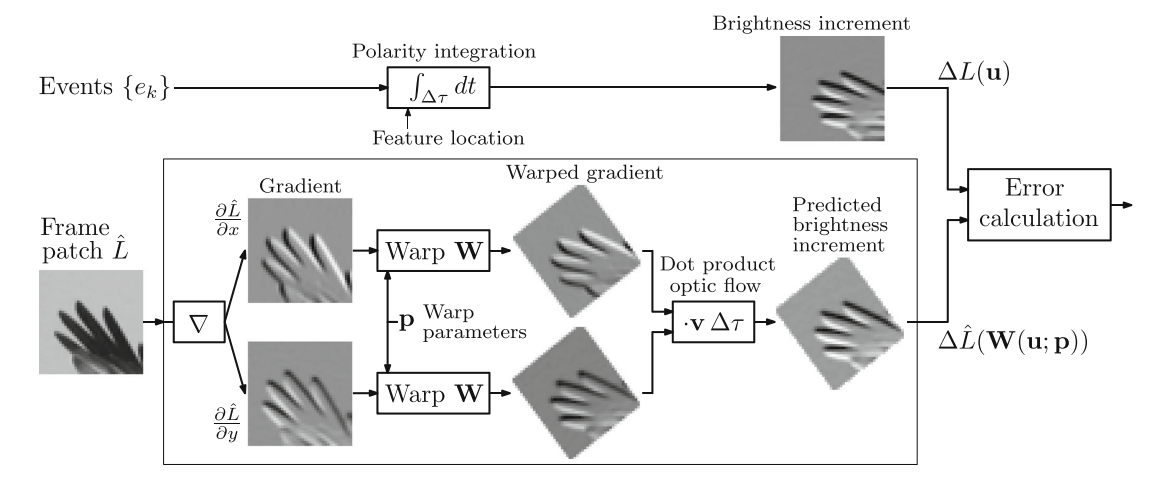
\includegraphics[width = 1\linewidth]{framework.png}
    \caption[Block diagram of EKLT]{Block diagram of EKLT, showing the comparison between brightness changes from images and events, from \cite{gehrig2020eklt}}
    \label{fig:sec2_eklt_block}
\end{figure}

It is worth noting, however, that the dependence on corners may present a problem for low-textured, or highly organic environments, where high quality corners are not always present.